\title{Survivable Set Connectivity}
\author{
 by Fermi Ma and Erik Waingarten
}
\date{\today}

\documentclass[12pt]{article}
\usepackage{amsmath}
\usepackage{amsthm}
\usepackage{amsfonts}
\usepackage{graphicx}
\usepackage{clrscode4e}
\usepackage{geometry}
 \geometry{
 a4paper,
 total={210mm,297mm},
 left=20mm,
 right=20mm,
 top=20mm,
 bottom=20mm,
 }

\newtheorem{proposition}{Proposition}
\newtheorem{definition}{Definition}
\newtheorem{lemma}{Lemma}

\begin{document}
\maketitle

\section{Introduction}

\subsection{Overview}

In this paper, we analyze the problem of Survivable Set Connectivity (SSC), a generalization of the classical Set Connectivity problem. Set connectivity is formulated as:
\begin{quote}
\textbf{Input}: A weighted graph $G = (V, E)$, with edge cost function $c: E \rightarrow \mathbb{R}^{\geq 0}$ and a collection of tuples of the form $(S_i, T_i)$. Each $(S_i,T_i)$ is a pair of disjoint vertex subsets. \\
\textbf{Output}: A minimum cost subgraph $H \subseteq G$ such that there is a path between $S_i$ and $T_i$ for each $i$. 
\end{quote}

Note that a ``path between $S_i$ and $T_i$" refers to any path that connects a vertex in $S_i$ to a vertex in $T_i$. The cost of a subgraph is simply the sum of the cost of the subgraph edges.

In SSC, the problem is modified so that each pair of sets $(S_i,T_i)$ must be connected by $k_i$ paths, instead of just 1. More formally, the problem is:

\begin{quote}
\textbf{Input}: A weighted graph $G = (V, E)$, with edge cost function $c: E \rightarrow \mathbb{R}^{\geq 0}$ and a collection of tuples of the form $(S_i, T_i)$, along with a value $k$. Again, each $(S_i,T_i)$ is a pair of disjoint vertex subsets. \\
\textbf{Output}: A minimum cost subgraph $H \subseteq G$ such that there are $k$ edge-disjoint paths between $S_i$ and $T_i$ for each $i$. 
\end{quote}

Unfortunately, solving exact Survivable Set Connectivity is $\mathsf{NP}$-hard \cite{ssc}. Therefore, the focus of this paper is on an approximate solution to a relaxation of this problem given in \cite{ssc}. Instead of requiring at least $k$ edge-disjoint paths between each pair, we require that each pair have at least $\Omega(\frac{k}{\log n})$ edge-disjoint paths, where $n = |V|$. With this relaxation, it is possible to find a subgraph with cost $O(polylog(n))$ times the optimum.

The paper is organized as follows. Sections 2, 3, and 4 provide the background necessary to understand the algorithm by Chalermsook et al. In Section 2, we present a natural integer linear programming formulation of the problem. Then, in Section 3, we introduce the idea of a \emph{tree embedding}, which allows us to transform arbitrary graphs $G$ into trees that can be more easily handled by the algorithm. In Section 4, we give a rounding scheme by Garg et al. known as RoundGKR, which the algorithm uses as a black box \cite{GKR}. We then pull together these concepts in Section 5 to present and analyze the approximation algorithm for SSC by Chalermsook et al. Finally, in Section 6, we present our own modification to the algorithm which improves the approximation ratio under special circumstances. We also conclude with ideas for potential further improvements.

\subsection{Related Work and Context}

The paper by Chalermsook et al. is the first and (currently) only paper to consider the Survivable Set Connectivity problem \cite{ssc}. Therefore, we survey the only known approximation algorithm for the problem. Chalermsook et al. noted that the original Set Connectivity problem has a large body of prior work, but they found that the best techniques for solving Set Connectivity do not translate to the survivable variant of the problem. Thus, we present Survivable Set Connectivity as a standalone problem, despite its obvious similarities to Set Connectivity.

At this time, it seems that Survivable Set Connectivity is motivated primarily by theoretical interest, as a ``natural" generalization of Set Connectivity. It is unknown if any common real-life graph problems are naturally formulated as a Survivable Set Connectivity problem.

\section{An Integer Linear Program}

In this section, we give an integer linear program that exactly solves SSC. Recall that the goal is to output a subgraph $H$ of $G$ such that each $(S_i,T_i)$ pair has at least $k$ edge disjoint paths. Naturally, we create an indicator variable $x_e$ for each edge based on whether or not it is included in $H$. 
\begin{align}
 x_e &= \left\{ \begin{array}{cc} 1 & e \in H \\
                                  0 & \text{ otherwise. } \end{array} \right.
\end{align}
Thus, our output $H$ will be the subgraph consisting of edges $e$ where $x_e = 1$. Also, for a graph $G = (V,E)$ and for a set $S \subseteq V$, we define $\delta(S)$ to be the set of edges crossing the cut from $S$ to $V \setminus S$. 
With this setup, we claim that the following ILP captures SSC exactly. 
\begin{align}
\min & \sum c(x) x_e  \\
\text{ s.t } & \sum_{e \in \delta(S)} x_e \geq k, \text{for each }S\text{ where } S_i \subset S,T_i \subset V \setminus S,  \\
& x_e \in \{0,1\} \text{ for all }e \in E
\end{align}

The objective function $\sum c(x) x_e$ simply minimizes the cost of all edges included in $H$. The constraint ensures that for all pairs $(S_i,T_i)$, any cut where $S_i$ is on one side of the cut and $T_i$ is on the other side has at least $k$ edges crossing the cut. We claim (but do not prove) that this property holds if and only if there are $k$ edge disjoint paths from $S_i$ to $T_i$. 

Of course, since this is an integer linear program, our best hope is to approximate it. We relax the program to fractional solutions, so the constraint that $x_e \in \{0,1\}$ becomes $0 \leq x_e \leq 1$. However, there is still a slight issue; we have exponentially many constraints. This occurs because there can be exponentially many choices of $S$ for each $(S_i,T_i)$ pair. To get around this issue, we note that the ellipsoid algorithm can handle linear programs with arbitrarily many constraints, as long as it is given a polynomial time separation oracle. Luckily, such an oracle exists and we sketch it here.

The oracle computes the minimum $S_i, T_i$ cut in the graph. It contracts $S_i$ and $T_i$ to single vertices, and then computes the min-cut in the remaining graph. If there is a min-cut of size less than $k$, then that cut will correspond to a violating contraint. If the min-cut has size at least $k$, then all cuts have size at least $k$, so all constraints are satisfied.

%The next tool we will need are tree embeddings. We have seen metric embeddings in class. Basically, we had a desired type of object $O$ (in the case of cuts, we had a metric space corresponding to a cut) what we did was come up with a metric space $(X, d)$ and a map $f: (X, d) \rightarrow O$ such that the map satisfied certain properties on the distances. 
%
%Here we will have a similar goal. We want to understand minimum cost weighted graphs, but since analyzing them is hard, we instead study minimum cost weighted trees, and then we map the trees back to the graphs. 
%
%\begin{definition}
%A tree embedding of a weighted graph $G = (V, E)$ will be a tree $T = (V_T, E_T)$ with weights $y: E \rightarrow \mathbb{R}^{\geq 0}$ and a function $\text{map} : V_T \cup E_t \rightarrow V \cup P(E)$ ($P(E)$ is the power set of $E$) such that
%\begin{align}
%\text{map}(V_t) &\subset V \\
%\text{map}(E_t) &\subset E
%\end{align}
%In other words, vertices map to vertices and edges map to edges. We will usually refer to an embedding as $(T, y, \text{map})$. 
%\end{definition}

\section{R\"{a}cke's Trees}
\label{sec:rackestrees}

In this section, we introduce a specific type of \emph{tree embedding}. A tree embedding is a transformation that takes general graphs and maps them to trees, while preserving much of the information present in the original graph. This way, algorithmic procedures that work well on trees can be applied to general graphs after a tree embedding has been applied. 

For the SSC problem, we will use a specific tree embedding formulated by R\"{a}cke, known as R\"{a}cke's trees. The property we are most interested in is the way that R\"{a}cke's tree embeddings preserve flow properties in the original graph. The definition of these embeddings is as follows.

\begin{definition}
For a given graph $G = (V, E)$ with edge capacities $x_e \geq 0$, $e \in E$, a R\"{a}cke's Tree embedding is a triple of the form $(T,y,\mathrm{map})$ where $T = (V_T,E_T)$ is a rooted tree, $y$ is a capacity function on the edges $E_T$ of $T$, and $\mathrm{map}$ is a function $V_T \cup E_T \to V \cup 2^E$ satisfying the following properties:
\begin{enumerate}
\item For each node $v \in V_T$, $\mathrm{map}(v) \in V$. Thus, the $\mathrm{map}$ function maps nodes in the tree $T$ to nodes in the original graph, $G$.
\item Furthermore, $\mathrm{map}$ restricted to the leaves of $T$ is a bijection with the vertices of $G$. In other words, each leaf of the tree $T$ is in one-to-one correspondence with a vertex of the original graph, $G$.
\item For each edge $e = (u,v) \in E_T$, $\mathrm{map}(e)$ is a set of edges that form a path between $\mathrm{map}(u)$ and $\mathrm{map}(v)$. Note that $\mathrm{map}(u)$ and $\mathrm{map}(v)$ are vertices in $G$, so $\mathrm{map}(e)$ specifies a set of edges in $G$.
%\item For some edge $e \in E_T$, $y_e$ (the cost of the edge) is a special quantity. Removing $y_e$ cuts the tree into two components, and so the leaves in the two components form a cut $\delta(S)$. Figure~\ref{fig:rackecut} gives an example for one such cut induced by an edge.
%\begin{align}
%y_e &= \sum_{e' \in \delta(S)} x_e
%\end{align}
\end{enumerate}
\end{definition}

With this setup, we can define the inverse function, $\mathrm{map}^{-1}$. If we try to compute $\mathrm{map}^{-1}(v)$ for some $v \in V$, we note that multiple vertices in $T$ could map to $v$. Thus, we specify that $\mathrm{map}^{-1}(v)$ be the unique \emph{leaf} vertex in $V_T$ that maps to $v$. We will also consider $\mathrm{map}^{-1}$ applied to sets of vertices $W \subseteq V$, and we define it in the obvious way: $\mathrm{map}^{-1}(W) = \bigcup_{v \in W} \mathrm{map}^{-1}(v)$.

For edges $e = (u,v) \in E$, we define $\mathrm{map}^{-1}(e) = \{ f \in E_T | e \in \mathrm{map}(f)\}$. This is simply the set of all edges $f$ in the tree $T$ that get mapped to a set of edges $\mathrm{map}(f)$ that contain $e$. Again, this defintiion can be extended to sets of edges $F \subseteq E$, so that $\mathrm{map}^{-1}(F) = \bigcup_{e \in F} \mathrm{map}^{-1}(e)$.

Finally, for an edge $e \in E_T$, we define $y_e$ as follows. The removal of $e$ from $T$ separates the tree into two connected components. Let $S$ be the set of vertices of $G$ mapped to by the leaves of one of the connected components, and so $V \setminus S$ is the set of vertices of $G$ mapped to by the leaves of the other connected component. Define $\delta(S)$ to be the set of edges in $E$ that cross from $S$ to $V \setminus S$. Then we set $y_e = \sum_{e' \in \delta(S)} x_{e'}$, the total edge capacity crossing the cut.

\begin{definition}
Given a R\"{a}cke tree, the load on an edge of the graph $e \in E$ is
\begin{align}
load(e) &= \sum_{f \in \text{map}^{-1}(e)} y_f,
\end{align}
and the relative load is defined as 
\begin{align}
rload(e) = \dfrac{load(e)}{x_e}.
\end{align}
\end{definition}

Figure~\ref{fig:racketree} shows an example R\"{a}cke's tree. We see a tree on the left-hand side which corresponds to the graph on the right-hand side. Each node is labeled by a number. The number indicates the projection of $\mathrm{map}$. A node of the tree labeled $1$ corresponds to the node in the graph labeled $1$. As you can see, the leaves are in bijection with the nodes of the graph. 

In addition, edges in the tree correspond to paths in the graph. The bolded edges of the tree map to the bolded edges in the graph. The top-most edge in the tree connects nodes $3$ and $5$, and that edge maps to the edge in the graph connecting $3$ and $5$. Then the bolded edge in the tree connecting $5$ to $5$ corresponds to the empty path. The bolded edge of the tree connecting $5$ to $4$ corresponds to the bolded edge in the graph connecting $4$ and $5$. Paths in the tree correspond to paths in the graph. 

We also note the capacity of the edge in the tree labeled $y$ is $x_1 + x_2 + x_3$. Edge $y$ disconnects the leaves into two groups, $S'$ and the rest. $S'$ maps bijectively to $S$. $S$ induces a cut on the graph, which cuts edges $x_1$, $x_2$, and $x_3$. Therefore, the capacity of $y$ (as defined by R\"{a}cke's trees) is the sum of the capacities of $x_1,x_2,$ and $x_3$. 

Another thing to notice is that $load(x_1) = 0$, since $\mathrm{map}^{-1}(x_1) = \emptyset$. An immediate consequence, which we can see from the load is that removing an edge with load 0 does not affect the connectivity of the graph. At a high level, the load will measure how necessary an edge is for connectivity. 

\begin{figure}
\label{fig:racketree}
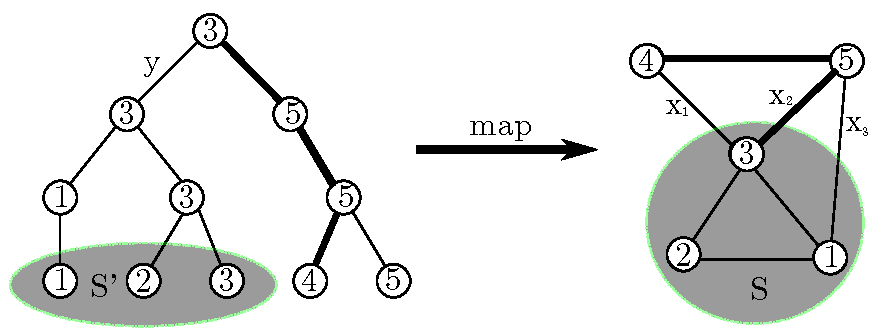
\includegraphics[width=\linewidth]{RackeTree.pdf}
\caption{A R\"{a}cke's tree example. A R\"{a}cke tree on the left maps to a graph on the right. The map on vertices is defined by the labelings on the nodes. The bolded edges map to the bolded edges. Edge $y$ defines a set of leaves $S'$, which defines a cut on the graph, $S$. $S$ cuts edges $x_1, x_2,$ and $x_3$; therefore, $y = x_1 + x_2 + x_3$.}
\end{figure}

The usefulness of R\"{a}cke's trees becomes apparent when we consider multi-commodity flows. Recall that the multi-commodity flow problem specifies $k$ different commodities, where each commodity $i$ must be routed from source $s_i$ to sink $t_i$, subject to constraints on the capacity of each edge. The resulting flow can be represented as a set of functions $\{ f_i \}$, where $f_i(e)$ is the nonnegative real number amount of commodity $i$ flowing on edge $e$. 

There is a natural way to map multi-commodity flows between $G$ and $T$. In particular, suppose we have a multi-commodity flow $\{ f_i \}$ on $G$. For each $i$, if there are $f_i$ units of flow going from $s_i$ to $t_i$ in $G$, we route $f_i$ units of flow in the $T$ from $\mathrm{map}^{-1}(s_i)$ to $\mathrm{map}^{-1}(t_i)$. If we are given a multicommodity flow $\{ f_i^T \}$ in $T$, then if we have $f_i^T(e)$ units of flow on edge $e$ in $T$, then we route $f_i^T(e)$ units of flow through the path $\mathrm{map}(e)$ in $G$ (recall that edges in $T$ map to paths in $G$).

There are some crucial properties of R\"{a}cke's trees which we will treat as black boxes. We will define these as lemmas without proof, and we refer to \cite{racke} for the proofs.

\begin{lemma}[\cite{racke}]
\label{lem:mapflows}
If we have a graph $G = (V, E)$ and capacities $x: E \rightarrow \mathbb{R}^{\geq 0}$ and a Racke tree $(T, y, \text{map})$. A multicommodity flow on $G$, $\{ f_i \}$, maps directly to a multicommodity flow on the tree which is also feasible. Likewise, a multicommodity flow on $T$ maps directly into a multicommodity flow on the graph, with the small caveat that we must multiply the capacity of the edge by the relative load. 
\end{lemma}

\begin{lemma}[\cite{racke}]
\label{lem:rload}
For some given graph $G = (V, E)$ and capacities $x: E \rightarrow \mathbb{R}^{\geq 0}$, we can sample efficiently from R\"{a}cke's trees of $G$, such that 
\begin{align}
\max_{e \in E} \textbf{E}[rload(e)] &\leq \alpha = O(\log n) 
\end{align}
\end{lemma}

\begin{lemma}[\cite{ssc}]
\label{thm:height}
The height of the trees sampled is $O(\log nC)$, where $C$ is the ratio of the largest to smallest capacity in $G$. In our cases, the height will always be $O(\log n)$. 
\end{lemma}

We refer to $\mathcal{D}$ as the distribution over R\"{a}cke trees with the above properties. In \cite{racke}, there is a polynomial time algorithm for sampling from this distribution.

\section{The RoundGKR Procedure}

The RoundGKR algorithm is a rounding procedure used to solve the Group Steiner Tree (GST) problem \cite{GKR}. The problem it stated as follows. \\

Group Steiner Tree:
\begin{quote}
\textbf{Input}: A tree $T = (V_T, E_T)$ rooted at $r$ where each edge has a nonnegative real value cost $c(e)$, along with a set $\{T_i\}$ where each $T_i \subseteq V_T$.\\
\textbf{Output}: The minimum cost subtree $H \subseteq T$ with a path from $r$ to $t_i$ for some $t \in T_i$ for all $i$.
\end{quote}

The following integer linear program solves the problem exactly:\\
GST-ILP:
\begin{align}
\min & \sum c(e) y_e  \\
\text{ s.t } & \sum_{e \in \delta(S)} y_e \geq 1, \text{ where } S_i \subset S, T_i \subset V - S, \delta(S) \text{ is the edges of the $S$ cut }
\end{align}

If we relax the integer linear program to a linear program and solve it, we can use RoundGKR to round the resulting fractional solution to an integer solution. The optimum to the linear program will assign fractional values in $[0,1]$ to each $y_e$. For any $e$, let $p(e)$ denote its parent edge (if it exists). We claim that since our problem is to find a subtree that includes the root $r$, edges that are closer to the root are at least as likely to be included in the subtree than edges farther from the root. Since the value of $y_e$ will be used as the probability that edge $e$ is included in $H$, we will assume that $y_{p(e)} \geq y_e$. 

The RoundGKR procedure simply starts at the root $r$ and builds the subtree $H$ by working its way down the original tree, $T$. It decides whether or not to include edge $e$ only once it has included edge $p(e)$ (if ever). At this step, it includes $e$ with probability $\frac{y_e}{y_{p(e)}}$. A simple inductive argment shows that an edge $e$ is chosen with probability $y_e$ (proof sketch: assume by induction that we know $Pr[\text{include $p(e)$}] = y_{p(e)}$. Then $Pr[\text{include $e$}] = Pr[\text{include $e$ $|$ include $p(e)$}]*Pr[\text{include $p(e)$}] = \frac{y_e}{y_{p(e)}}y_{p(e)} = y_e$.)

The important property of the algorithm can be summarized in the following lemma, whose proof can be found in \cite{GKR}.

\begin{lemma}[\cite{GKR}]
\label{lem:findpath}
Suppose that $T = (V_t, E_t)$ support a flow of at least $1$ from $T_i$ to the root $r$ without the edges $F_t$. Then the RoundGKR returns a solution with a path in $T$ from $T_i$ to $r$ without using $F_t$ with probability at least $\Omega(\frac{1}{\log n})$. 
\end{lemma}

We will rely on this lemma heavily. In fact, since we need $\Omega(\frac{k}{\log n})$ edge-disjoint paths, we will argue that if we let $F_t$ be any set of at most $\Omega(\frac{k}{\log n})$ edges, then we still have a path, and therefore, we have $\Omega(\frac{k}{\log n})$ paths.  

\section{Algorithm}

Now we will combine the ideas of the linear program to approximate a solution to Survivable Set Connectivity. We copy the algorithm as it is written in the paper below, although we will separate the algorithm into parts and explain each part in detail.
\begin{codebox}
\li Set $H \leftarrow \emptyset$
\li Compute linear program SSC-LP and set to zero any $x_e < \dfrac{k}{n^2}$.
\li Let $x' \leftarrow x*\frac{4}{k}$. 
\li Prepare $\mathcal{D}$ be the distribution of R\"{a}cke's tree embeddings for $G$ with $x'$.
\li \For $\tau$ rounds \Do
\li Sample $(T, y, \text{map})$ from $\mathcal{D}$. 
\li \For $q = 0, ..., 2\log n$ \Do
\li \For $v \in V_t$ \Do
\li With probability $\min\{1, \dfrac{4}{2^q}\}$, $q$-mark $v$
\li \If $v$ is $q$-marked \Then
\li Set $y^{v, q}\leftarrow 2^{q+1}y$ and $E^{v,q} \leftarrow \emptyset$.
\li \For $\tau'$ iterations, \Do
\li $E^{v,q} \leftarrow E^{v,q} \cup$ RoundGKR$(T_v, v, y^{v,q})$ \End
\li $H \leftarrow H \cup \text{map}(E^{v,q})$ \End \End \End \End
\li return $H$
\end{codebox}

\subsection{Algorithm Idea}

Here, we provide an intuitive explanation of the algorithm as well as the main motivations for each procedure. Of course, we will revist these ideas in the analysis.

After running the linear program, we rescale $x$ to $x'$ by a $\frac{4}{k}$ factor, which ensures that we have a flow of at least $4$ in each $(S_i, T_i)$. This flow of $4$ will correspond to a flow of $4$ in the R\"{a}cke's trees.

The RoundGKR algorithm is the main tool used for our rounding scheme. RoundGKR finds paths in trees which avoid specific edges with probability $\Omega(\frac{1}{\log n})$ (this is Lemma~\ref{lem:findpath}) given there is sufficient flow. We repeat this $\tau' = O(\log n)$ times to assure a constant probability of finding such paths. 

However, we can only run RoundGKR on trees, not general graphs. We introduce the R\"{a}cke's tree embedding specifically for this purpose. We know a flow of $4$ exists between leaves (Lemma~\ref{lem:mapflows}). Each flow path will go up the tree to some ancestor $v$ and then back down to a leaf. One such path might be found when $v$ gets marked. One path will go to $s_i'$ and one to $t_i'$.

Lemma~\ref{lem:findpath} requires us to have a flow of at least $1$ avoiding some edges. If a flow path from $s_i'$ to $t_i'$ goes through ancestor $v$ and carries a flow of value $f$, we can apply the lemma if $f \geq 1$. We scale the capacities by $2^{q+1}$ in order to search for the flow value. We only scale with probabilities $\dfrac{4}{2^q}$ so our costs does not increase by more than $O(\log n)$. Figure~\ref{fig:roundgkronnode} shows how a flow path might be found.

\section{Algorithm Analysis}

\subsection{Overview}

We claim that the algorithm finds a solution which has
\begin{itemize}
\item (Claim A) cost within a polylogarithmic factor of the optimum
\item (Claim B) at least $\Omega(\frac{k}{\log n})$ edge disjoint paths between each $(S_i, T_i)$ pair
\end{itemize}

We first prove Claim A assuming that Claim B is true, and then we prove claim B.


\subsection{Claim A}

\begin{lemma}[\cite{ssc}]
\label{lem:cost}
$\textbf{E}[c(H)] = O(\log^4n(\frac{\log h}{k}+1)) * c(x)$, where $c(x) = \sum_e c(e)x_e$. 
\end{lemma}

\begin{proof}
We prove this by bounding the probability that a given edge is included in $H$ by $O(\log^4n(\frac{\log h}{k} + 1))x_e$. The claim then follows by linearity of expectation.

Let $(T = (V_t, E_t), y, \text{map})$ be a R\"{a}cke's tree sampled from $\mathcal{D}$. For an edge $e$ to be included in our output subgraph $H$, there must have been some tree edge $e' \in E_T$ that maps to $e$ (so $e \in \mathrm{map}(e')$) selected to be in $E^{v,q}$ for some vertex $v \in V_t$ and some index $q \in [0,\dots,2\log n]$. For this to occur, $v$ must be $q$-marked, an event that occurs with probability $\frac{4}{2^{q}}$. 

For a given edge $e'$, there are at most $height(T)$ ancestors, which means that there are at most $height(T)$ different vertices $v$ that, if $q$-marked, may lead to $e'$ being included. For each $v$, we must consider all $O(\log n)$ possible values of $q$. For each value of $q$, the probability of being $q$-marked is $\frac{4}{2^{q}}$. Once the vertex is $q$-marked, we have $\tau'$ trials of the RoundGKR algorithm, where in each trial, there is a $2^{q+1}y_{e'}$ chance of edge $e'$ being included (by construction of the algorithm). Multiplying these probablities together and applying a union bound over all $\tau'$ trials and over all possible values of $q$, we get an upper bound of 

\begin{align}
height(T) \sum_{q=0}^{2\log n} \frac{4}{2^{q}} 2^{q+1} y_{e'} \tau' &= height(T) \tau' y_{e'} \sum_{q=0}^{2\log n} 8 = O(\log^3 n) y_{e'} 
\end{align}

So the probability that a given edge of the tree is included in a particular sampling of a R\"{a}cke's tree is $O(\log^3 n) y_{e'}$. 

Using this, we can bound the probability that a particular edge $e$ of the original graph is included. For $e$ to be included, on one of the $\tau$ trials, the algorithm must chose some tree edge $e'$ such that $e' \in \mathrm{map}^{-1}(e)$ (recall that this is the set of tree edges which, if selected, result in edge $e$ being included). So let $X_e$ be the indicator random variable which says that edge $e$ is included in $H$. Then we have the inequality
\begin{align}
 \textbf{E}_{R}[X_e] &\leq \tau \sum_{e' \in \mathrm{map}^{-1}(e)} O(\log^3 n) y_{e'} 
\end{align}
where the expectation $\text{E}_{R}[X_e]$ is over the random choices of the algorithm, after choosing a R\"{a}cke tree. The $\tau$ comes from a union bound over all trials. The $O(\log^3 n)y_{e'}$ comes from the first part of the proof, where we bounded the probability of including a specific $e'$. 

To simplify this inequality, we apply a series of definitions and lemmas stated earlier in Section~\ref{sec:rackestrees}. 
\begin{align}
\textbf{E}_{\mathcal{D}}[E_{R}[X_e]] &\leq \textbf{E}_{\mathcal{D}}[\tau \sum_{e' \in \mathrm{map}^{-1}(e)} O(\log^3 n) y_{e'}] \\
               &\leq O(\log^3 n) \tau \textbf{E}_{\mathcal{D}}[\sum_{e' \in \mathrm{map}^{-1}(e)} y_{e'}] \\
               & \leq O(\log^3 n) \tau \textbf{E}_{\mathcal{D}}[load(e)]
\end{align}
where the expectation is over the choice of R\"{a}cke tree. Using the definition of $rload$, 
\begin{align}
\textbf{E}[X_e] &\leq O(\log^3 n) \tau E[rload(e) x_e'] \\
                &\leq O(\log^3 n) \tau \frac{4}{k} \alpha x_e
\end{align}
where $\text{E}[X_e]$ is the expectation over both random choices of the algorithm as well as random choices of the R\"{a}cke tree. Lemma~\ref{lem:rload} gives a bound on the maximum relative load. $\alpha$ is bounded by $O( \log n)$, so our final inequality is 
\begin{align}
 \textbf{E}[X_e] &\leq \frac{O(\log^4 n)\tau}{k} x_e 
\end{align}

From here, we simply apply linearity of expectation to bound the total cost. We have 
%
%
% Above, we argued that $E[Y_{e'}] \leq O(\log^3 n)y_{e'}$.
%\begin{align}
%X_e \leq \sum_{e' \in \text{map}(e)} Y_{e'}
%\end{align}
%Because if $e$ is included in the graph, it must have come from some edge in the tree. 
%\begin{align}
% \textbf{E}[X_e] &\leq \tau \sum_{e' \in \text{map}^{-1}(e)} O(\log^3 n) y_{e'} \\
%        &= O(\log^3 n) \tau \textbf{E}[load(e)] \\
%        &= O(\log^3 n) \tau \textbf{E}[rload(e)x_e'] \\
%        &\leq O(\log^3 n) \tau \dfrac{4}{k} \alpha x_e\\
%        & = \dfrac{O(\log^4 n)\tau}{k} x_e
%\end{align}
%So now, bounding the optimum, we get
\begin{align}
\textbf{E}[c(H)] &= \sum_{e \in E} c(x_e)\textbf{E}[X_e] \\
                 &\leq \dfrac{O(\log^4 n)\tau}{k} \sum_{e \in E} c(x_e) x_e
\end{align}
So when $\tau = O(\log h + k)$, we get our desired approximation.
\end{proof}

\begin{figure}
\label{fig:roundgkronnode}
\centering
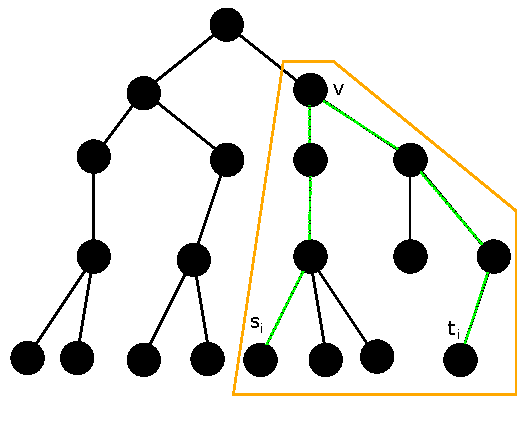
\includegraphics[width=0.6\linewidth]{RoundGKRonNode.pdf}
\caption{Execution of GKR on some subtree rooted at $v$ in a particular round finding paths to $s_i$ and $t_i$.}
\end{figure}

Having established that the expected cost is only a polylogarithmic factor away from the optimum, it remains to show that the edges chosen do in fact form a graph which connects $(S_i, T_i)$ with $\Omega(\frac{k}{\log n})$ disjoint paths for each $i$. We will need the following definition.


\subsection{Claim B}

\begin{definition}
For some set of edges $F \subseteq E$, the sampled tree embedding, $(T, y, \text{map})$ is bad if $F_T = \text{map}^{-1}(F)$ 
\[ \sum_{e' \in F_T} y_{e'} \geq \frac{1}{2} \]
And good otherwise.
\end{definition}

Intuitively, bad sets correspond to sets which are necessary in the graph. We want graphs to be good with respect to sets of size $\Omega(\frac{k}{\log n})$ in order to ensure connectivity even if we remove them.

\begin{lemma}[\cite{ssc}]
\label{lem:notbad}
Fix some $F$ of size at most $\dfrac{k}{16 \alpha}$. Then the probability that a sampled tree embedding $(T, y, \text{map})$ from $\mathcal{D}$ is bad is at most $\frac{1}{2}$. 
\end{lemma} 

\begin{proof}
Suppose we have a bad embedding for the set $F$. Then 
\begin{align}
\sum_{e \in F} load(e)&= \sum_{e \in F} \sum_{e' \in \text{map}^{-1}(e)} y_{e'} \\
                    &\geq \sum_{e' \in F_T} y_{e'} \\
                    &\geq \frac{1}{2}
\end{align}
Where the first inequality we get from taking the sum over the union versus the disjoint union, and the second inequality from the assumption that the tree embedding is bad. 

Therefore, a bad tree means that the load of the set of $F$ is more than $\frac{1}{2}$. Therefore,
\begin{align}
Pr[\text{pick a bad tree for $F$}] &\leq Pr[ \sum_{e\in F} load(e) \geq \frac{1}{2}]
\end{align}
From Lemma~\ref{lem:rload}, we know that
\begin{align}
\textbf{E}[ \sum_{e \in F} load(e) ] &\leq \sum_{e \in F} \textbf{E}[rload(e)]x_{e'} \\
                                   & \leq \sum_{e\in F} \alpha \frac{4}{k} x_{e} \\
                                   & \leq \dfrac{4\alpha}{k} |F| \\
                                   &\leq \frac{1}{4}
\end{align}
Since we limited the size of $F$. Now invoking Markov's inequality, we know that the probability of bad event is at most $\frac{1}{2}$. 
\end{proof}

\begin{lemma}[\cite{ssc}]
\label{lem:connected}
With probability at least $\frac{3}{4}$, all set pairs are at least $\frac{k}{16\alpha} + 1$ edge connected in $H$. 
\end{lemma}

\textbf{Proof Idea of Lemma~\ref{lem:connected}}:
\begin{enumerate}
\item Set a particular set of edges $F$ of size at most $\Omega(\dfrac{k}{\log n})$. 
\item Argue that with probability at most $\frac{1}{2}$, the edges in $F$ are not necessary for connectivity by claiming that the total $load$ on the edges in low. (This is Lemma~\ref{lem:notbad}). 
\item We will condition on this probability to show that if we remove $\text{map}(F)$ on the tree, we still have sufficient flow from each $s_i$ to $t_i$. Each flow path must go up the tree to some common ancestor $v$ and then back down.
\item Then we will claim that at some $v$, it gets marked and the RoundGKR algorithm which is rooted at $v$ finds the two paths from $v$ to $s_i$ and $t_i$, and so the path will be included with sufficient probability and exclude $F$.
\item We finally union bound over all $F$ and over all $i$ to show that we succeed with constant probability. 
\end{enumerate}

\begin{proof}[Proof of Lemma~\ref{lem:connected}]
We fix an $F$ of size at most $\frac{k}{16\alpha}$ and an $i$ and show that $(S_i, T_i)$ are connected with an edge outside of $F$. I will show this happens with a probability at least $\beta$. So the probability of failure is $(1-\beta)$. If we repeat this $\tau = \frac{1}{\beta}\ln(4hn^{\frac{k}{16\alpha}}) = O(\log h + k)$ times, then our failure probability goes down to $\dfrac{1}{4hn^{\frac{k}{16\alpha}}}$. So now we take the union bound over all of $F$ and over all $i$, so we get probability of failure at most $\frac{1}{4}$.

It remains to show that the probability that we find a path from $S_i$ to $T_i$ without using the edges from $F$ is at least $\beta$. We do this in the following lemma.
\end{proof}

As of right now, we have shown steps $1$, $2$ and $5$ in the proof idea of Lemma~\ref{lem:connected}. We finish the proof by showing steps $3$ and $4$. 

\begin{lemma}
Fix some $F$ and some $i$, where $|F| < \dfrac{16k}{\alpha}$. The probability that at round $t$ we find a path from $S_i$ to $T_i$ without using edges from $F$ is at least some constant $\beta > 0$. 
\end{lemma}

\begin{proof}
We condition on the probability that $F$ is good at round $t$, which by Lemma~\ref{lem:notbad} is at least $\frac{1}{2}$. Now we can set the $y$ terms of $F_T = \text{map}^{-1}(F)$ to zero, in order to avoid picking an edge in $F$. 

Since we have a good embedding with respect to $F$. The assumption was that $G$ can support a flow of at least $k$ in the original graph (by the solution to the fractional linear program). Recall that we reweighed the values $x$ by $\frac{4}{k}$, so we can support a flow of at least $4$ in the original graph with $x'$. So by Lemma~\ref{lem:mapflows}, $T$ supports a flow from $S_i' = \text{map}^{-1}(S_i)$ to $T_i' = \text{map}^{-1}(T_i)$ of value at least $4$. 

Removing the total capacity of $\frac{1}{2}$, we are left with a flow of $2 - \frac{1}{2} = \frac{3}{2}$. In particular, we can support a unit flow from $S_i'$ to $T_i'$. That unit flow can be decomposed into paths $P_1, ..., P_z$, disregarding paths with very small amount of flow $(\leq \frac{1}{2n^2})$. Each flow path goes up from a leaf, turns at some $v$, and then goes down to another leaf. Let $\phi_v$ be the flow turning at $v$. Let $\phi_v$ be the total flow turning at node $v$. 

Since we support a flow of at least $\frac{3}{2}$ and we removed paths with at most $\frac{1}{2n^2}$ flow, we are left with
\[ \sum_{v \in V_t} \phi_v \geq \frac{3}{2} - \dfrac{1}{2n^2}|E_t| \geq 1 \]
Now $\phi_v$ falls between some $(2^{-q_v-1}, 2^{-q_v}]$ for some $q_v \in \{0, ..., 2\log_2 n\}$. Now the probability that none of the $v \in V_t$ is $q$-marked exactly at $q_v$ when we have a good embedding is at most $e^{-3/4}$ which follows by a Chernoff bound. The important thing to note is that each time we try to $q$-mark a node, it is an independent event. The expected value of the number of vertices that get $q$-marked at $q_v$ is at least $4$ and we need at least $1$. These values are sums of independent random variables, so we can apply the Chernoff bound.

Conditioning on finding one such $v$, the path gets multiplied by $2^{q_v+1}$. Now it supports a flow of $1$. Lemma~\ref{lem:findpath} says the path will be included with probability at least $\Omega(\frac{1}{\log n})$ in a single round of RoundGKR. So if we repeat it $\tau'$ times, the probability we do not find the path is $1 - (1 - \Omega(1/\log n))^{\tau'}$. Letting $\tau' = O(\log n)$, we get any constant probability $\epsilon$. Since we need to find both paths from the root to both leaves, we get a failure probability of $2\epsilon$.

So the probability that we find a path outside of $F$ is at least one minus the union bound over failure probabilities. This is $1 - \frac{1}{2} - e^{-3/4} - 2\epsilon > 0$. 
\end{proof}

This concludes steps $3$ and $4$ of the proof idea for Lemma~\ref{lem:connectivity}. This finishes the proof that after running the rounding algorithm, each $(S_i, T_i)$ tuple will have $\Omega(\frac{k}{\log n})$ paths connecting $S_i$ to $T_i$. 

\section{Potential Improvements}

There seems to be a trade off in the algorithm between finding flow paths between many groups at once and searching for nodes the flow paths traverse. In the original algorithm, we must iterate through each $v \in V_T$ and run some RoundGKRrounds on its subtree. If there are multiple flow paths from different groups, say $(S_1', T_1')$ and $(S_2', T_2')$ going through $v$, then the original algorithm could find both at once. We could be finding $h$ paths with $O(\log n)$ cost (since running RoundGKR on each subtree makes each edge appear in $O(\log n)$ subtrees). 

If we know $\sum_{i=1}^h |S_i| = S$ is small (the number of sources is small). We can run the algorithm without looking for the nodes where the flow paths turn. In particular, we could treat it as many different instances of the Group Steiner Tree problem. The algorithm would be:
\begin{codebox}
\li Set $H \leftarrow \emptyset$
\li Compute linear program SSC-LP and set to zero any $x_e < \dfrac{k}{n^2}$.
\li Let $x' \leftarrow x*\frac{4}{k}$. 
\li Let $\mathcal{D}$ be the distribution of R\"{a}cke's tree embeddings for $G$ with $x'$.
\li \For $\tau$ rounds \Do
\li Sample $(T, y, \text{map})$ from $\mathcal{D}$. 
\li \For $q = 0, ..., 2\log n$ \Do
\li \For \For $i \in [h]$ and $s \in S_i'$ \Do
\li With probability $\min\{1, \dfrac{4}{2^q}\}$, $q$-mark $s$
\li \If $s$ is $q$-marked \Then
\li Set $y^{s, q}\leftarrow 2^{q+1}y$ and $E^{s,q} \leftarrow \emptyset$.
\li \For $\tau'$ iterations, \Do
\li $E^{s,q} \leftarrow E^{s,q} \cup$ RoundGKR$(T_s, s, y^{s,q})$ \End
\li $H \leftarrow H \cup \text{map}(E^{s,q})$ \End \End \End \End
\li return $H$
\end{codebox}
The main difference lies in line 8. Instead of iterating through all $v \in V_T$ to find where the flow path turns, we take advantage of knowing where the flow begins. We know all flow paths go from $S_i'$ to $T_i'$, so we make $s \in S_i'$ the root of the tree. It is unnecessary to look for where the flow turns. We still have to iterate through $q= 0, ..., 2\log n$, since the flow of at least $1$ between $S_i'$ and $T_i'$ might be divided among different flow paths starting at different nodes in $S_i'$. This gets rid of the $O(\log n)$ factor in the cost because of the height, and adds a factor of $S$.

Lemma~\ref{lem:connected} still holds. Since we know exactly where the flow paths must start.

\begin{lemma}
The above algorithm has $\textbf{E}[c(H)] = O(S\log^3 n(\dfrac{\log h}{k} + 1))*c(x)$.
\end{lemma}

\begin{proof}
The proof is the same as the proof of Lemma~\ref{lem:cost}. The only difference is that instead of each edge being included in at most $height(T)$ RoundGKR steps, we include it in at most $S$ RoundGKR steps. 
\end{proof}

Therefore, if $S = o(\log n)$, it is better to run this modified algorithm. Along similar lines, if $\sum_{i \in [h]} |T_i| = T$ is small, then we could compress the R\"{a}cke tree to contain only the leaves we want. If $T = O(\log n)$, then the tree could be compressed to size $O(\log n)$, and so we would find unit flow paths with probability $\Omega(\frac{1}{\log \log n})$. This means we could reduce $\tau'$ to $O(\log \log n)$ and decrease our approximation ratio.

Now the question becomes, can we reduce $S$ to $h$? One possible idea is to join all the nodes in $S_i'$. This would destroy the tree property for RoundGKR, but maybe we can disregard some cycles (at least if we analyzed the case with unit costs on the edges). \cite{ssc} uses RoundGKR and R\"{a}cke trees as black boxes, so maybe there is some hope. If this is possible, then our competitiveness would be $O(h\log^3n(\dfrac{\log h}{k} + 1))$. Now if $h = o(\log n)$, then we would prefer this algorithm.

\bibliography{references}
\bibliographystyle{splncs}

\end{document}